\section{Постановка задачі}

Метою є мінімізація функції, що називається енергією.
В першій роботі Бланца и Феттера \cite{blanz:romdhani:vetter}
енергія складалася з
суми квадратів різниць кольорів пікселів
оригінального та синтезованого зображення,
суми квадратів параметрів, що мають нормальний розподіл,
та суми квадратів відхилень параметрів камери від початкових значень,
що визначалися оператором:
\begin{equation}\label{eq:energy:blanz}
  E_N\left( x, \theta \right)
  = \sum_{i \in I' \subset I}
      \frac{\left\| y_i \right\|^2}{\sigma^2_N}
  + \sum_{j = 1}^{n} x_j^2
  + \sum_{k = 1}^{m}
      \frac{\left\| \theta_m - \overline{\theta_m} \right\|^2}
           {\sigma^2_{\theta_m}}.
\end{equation}
Дисперсія $\sigma_N^2$ відповідає шуму на оригінальному зображенні.
Зауважимо, що беруться не всі пікселі зображення,
а тільки ті, що відповідають пікселям, де намальовано модель.
Щоб кількість доданків завжди була однаковою,
на кожній ітерації алгоритму випадковим образом
обирається певна кількість трикутників
з ймовірністю, що пропорційна до їх площі.

Процедура мала наступний вигляд:
\begin{enumerate}
  \item на перших кроках використовується модель
    з меншою кількістю трикутників та вершин;
  \item спочатку використовуються лише параметри камери
    та найзначущі параметри моделі (перші головні компоненти),
    і поступово додаються нові компоненти;
  \item спочатку $\sigma_N$ обирається достатньо великим,
    аби збільшити апріорну ймовірність параметрів моделі,
    а з кожною ітерацією його зменшують,
    щоб отримувати все більш схоже зображення.
\end{enumerate}

У новітніх роботах для кращих результатів реконструкції використовуються
додаткові відомості про обличчя --- опорні точки.
Знаходження особливих точок на зображенні голови
являє собою окрему складну задачу.
Одним з популярніших на даний час є метод, опублікований в статті
``вирівнювання обличчя за одну мілісекунду'',
що використовується в бібліотеці з відкритим кодом dlib \cite{Kazemi:2014}.
Результати, що дає алгоритм, можна побачити на рис. \ref{fig:problems:dlib}.
\begin{figure}[h]
  \centering
    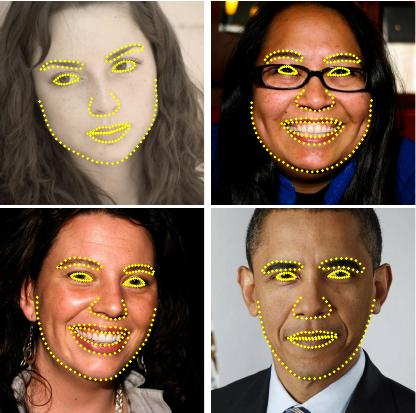
\includegraphics[width=0.5\textwidth]{images/dlib}
  \caption{Приклади знаходження опорних точок обличчя}
  \label{fig:problems:dlib}
\end{figure}

Окрім того,
замість суми квадратів відхилень використовується зміщена оцінка дисперсії.
Це дозволяє брати різну кількість точок на кожній ітерації.
Нова цільова функція має вигляд
\begin{equation}\label{eq:energy:face2face}
  E\left( x, \theta \right)
  = \omega_c \cdot \sum_{i \in I' \subset I} \frac{y_i^2}{\left| I' \right|}
  + \omega_r \cdot \sum_{j = 1}^{n} x_j^2
  + \omega_l \cdot \sum_{l \in L} \frac{\Delta_l^2\left( x \right)}
                                       {\left| L \right|},
\end{equation}
де $\Delta_l$ --- функція,
яка перетворює параметри моделі на відхилення її опорних точок від реальних.
Коефіцієнти $\omega_c$, $\omega_r$ і $\omega_l$
обираються рівними $1$, $2.5 \cdot 10^{-5}$ і $10$ відповідно.
